\subsection{Interrelación Titulación - Asignatura}

   \begin{description}
      \item[Definición] En esta interrelación se deja constancia de que cada
      titulación establecida en el sistema podrá disponer de varias asignaturas.

      \begin{itemize}
       \item Una titulación puede disponer de varias asignaturas.
       \item Una asignatura solamente puede pertenecer a una determinada
             titulación.
      \end{itemize}

      \item[Características] La interrelación presenta las siguientes
                             características:

         \begin{itemize}
            \item \textbf{Nombre:} T-A
            \item \textbf{Tipo de la interrelación:} El tipo de entidad
                  Asignatura es débil por identificación respecto al tipo de
                  entidad Titulación.
            \item \textbf{Cardinalidad de la interrelación:} 1:N
                  \begin{itemize}
                     \item Titulación: dispone\_de (0,n)
                     \item Asignatura: pertenece\_a (1,1)
                  \end{itemize}
            \item \textbf{Número de atributos:} Ninguno.
         \end{itemize}

      \item[Diagrama] La figura \ref{diagramaT-A} muestra el diagrama de la
                      interrelación.

      \item \begin{figure}[!ht]
            \begin{center}
            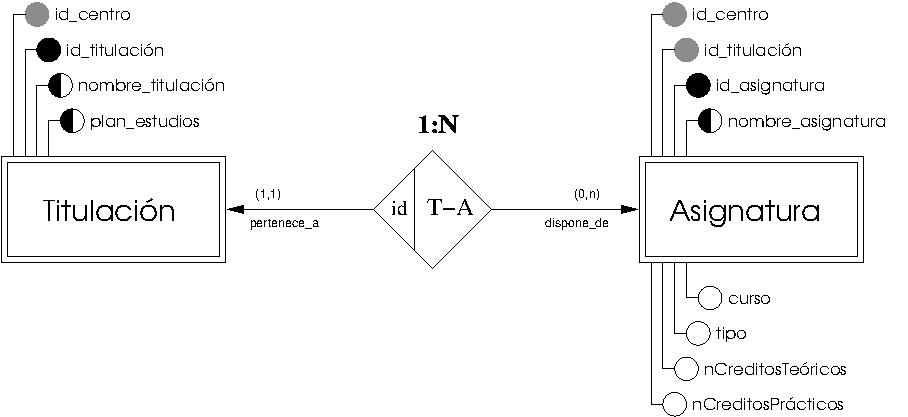
\includegraphics[]{07.Modelo_Entidad-Interrelacion/7.3.Analisis_Interrelaciones/diagramas/T-A.pdf}
            \caption{Diagrama de la interrelación T-A.}
            \label{diagramaT-A}
            \end{center}
         \end{figure}

      \item[Ejemplo práctico del tipo de interrelación]

      \item \begin{center}
            \begin{tabular}{ | r r | }
            \hline
            \multicolumn{2}{ | c | }{\textbf{Tipo de interrelación T-A}} \\
            \hline
            \textbf{Titulación} & \\
            id\_centro & 15 \\
            id\_titulación & 3 \\
            \hline
            \textbf{Asignatura} & \\
            id\_centro & 15 \\
            id\_titulación & 3 \\
            id\_asignatura & 17 \\
            \hline
            \end{tabular}
         \end{center}
   \end{description}
